\documentclass[twoside]{book}

% Packages required by doxygen
\usepackage{calc}
\usepackage{doxygen}
\usepackage{graphicx}
\usepackage[utf8]{inputenc}
\usepackage{makeidx}
\usepackage{multicol}
\usepackage{multirow}
\usepackage{textcomp}
\usepackage[table]{xcolor}

% Font selection
\usepackage[T1]{fontenc}
\usepackage{mathptmx}
\usepackage[scaled=.90]{helvet}
\usepackage{courier}
\usepackage{amssymb}
\usepackage{sectsty}
\renewcommand{\familydefault}{\sfdefault}
\allsectionsfont{%
  \fontseries{bc}\selectfont%
  \color{darkgray}%
}
\renewcommand{\DoxyLabelFont}{%
  \fontseries{bc}\selectfont%
  \color{darkgray}%
}

% Page & text layout
\usepackage{geometry}
\geometry{%
  a4paper,%
  top=2.5cm,%
  bottom=2.5cm,%
  left=2.5cm,%
  right=2.5cm%
}
\tolerance=750
\hfuzz=15pt
\hbadness=750
\setlength{\emergencystretch}{15pt}
\setlength{\parindent}{0cm}
\setlength{\parskip}{0.2cm}
\makeatletter
\renewcommand{\paragraph}{%
  \@startsection{paragraph}{4}{0ex}{-1.0ex}{1.0ex}{%
    \normalfont\normalsize\bfseries\SS@parafont%
  }%
}
\renewcommand{\subparagraph}{%
  \@startsection{subparagraph}{5}{0ex}{-1.0ex}{1.0ex}{%
    \normalfont\normalsize\bfseries\SS@subparafont%
  }%
}
\makeatother

% Headers & footers
\usepackage{fancyhdr}
\pagestyle{fancyplain}
\fancyhead[LE]{\fancyplain{}{\bfseries\thepage}}
\fancyhead[CE]{\fancyplain{}{}}
\fancyhead[RE]{\fancyplain{}{\bfseries\leftmark}}
\fancyhead[LO]{\fancyplain{}{\bfseries\rightmark}}
\fancyhead[CO]{\fancyplain{}{}}
\fancyhead[RO]{\fancyplain{}{\bfseries\thepage}}
\fancyfoot[LE]{\fancyplain{}{}}
\fancyfoot[CE]{\fancyplain{}{}}
\fancyfoot[RE]{\fancyplain{}{\bfseries\scriptsize Generated on Thu Nov 19 2015 21\-:03\-:09 for My Project by Doxygen }}
\fancyfoot[LO]{\fancyplain{}{\bfseries\scriptsize Generated on Thu Nov 19 2015 21\-:03\-:09 for My Project by Doxygen }}
\fancyfoot[CO]{\fancyplain{}{}}
\fancyfoot[RO]{\fancyplain{}{}}
\renewcommand{\footrulewidth}{0.4pt}
\renewcommand{\chaptermark}[1]{%
  \markboth{#1}{}%
}
\renewcommand{\sectionmark}[1]{%
  \markright{\thesection\ #1}%
}

% Indices & bibliography
\usepackage{natbib}
\usepackage[titles]{tocloft}
\setcounter{tocdepth}{3}
\setcounter{secnumdepth}{5}
\makeindex

% Hyperlinks (required, but should be loaded last)
\usepackage{ifpdf}
\ifpdf
  \usepackage[pdftex,pagebackref=true]{hyperref}
\else
  \usepackage[ps2pdf,pagebackref=true]{hyperref}
\fi
\hypersetup{%
  colorlinks=true,%
  linkcolor=blue,%
  citecolor=blue,%
  unicode%
}

% Custom commands
\newcommand{\clearemptydoublepage}{%
  \newpage{\pagestyle{empty}\cleardoublepage}%
}


%===== C O N T E N T S =====

\begin{document}

% Titlepage & ToC
\hypersetup{pageanchor=false}
\pagenumbering{roman}
\begin{titlepage}
\vspace*{7cm}
\begin{center}%
{\Large My Project }\\
\vspace*{1cm}
{\large Generated by Doxygen 1.8.6}\\
\vspace*{0.5cm}
{\small Thu Nov 19 2015 21:03:09}\\
\end{center}
\end{titlepage}
\clearemptydoublepage
\tableofcontents
\clearemptydoublepage
\pagenumbering{arabic}
\hypersetup{pageanchor=true}

%--- Begin generated contents ---
\chapter{Hierarchical Index}
\section{Class Hierarchy}
This inheritance list is sorted roughly, but not completely, alphabetically\-:\begin{DoxyCompactList}
\item \contentsline{section}{Abstract\-Cell}{\pageref{classAbstractCell}}{}
\begin{DoxyCompactList}
\item \contentsline{section}{Conway\-Cell}{\pageref{classConwayCell}}{}
\item \contentsline{section}{Fredkin\-Cell}{\pageref{classFredkinCell}}{}
\end{DoxyCompactList}
\item \contentsline{section}{Cell}{\pageref{classCell}}{}
\item \contentsline{section}{Life$<$ T $>$}{\pageref{classLife}}{}
\end{DoxyCompactList}

\chapter{Class Index}
\section{Class List}
Here are the classes, structs, unions and interfaces with brief descriptions\-:\begin{DoxyCompactList}
\item\contentsline{section}{\hyperlink{classAbstractCell}{Abstract\-Cell} }{\pageref{classAbstractCell}}{}
\item\contentsline{section}{\hyperlink{classCell}{Cell} }{\pageref{classCell}}{}
\item\contentsline{section}{\hyperlink{classConwayCell}{Conway\-Cell} }{\pageref{classConwayCell}}{}
\item\contentsline{section}{\hyperlink{classFredkinCell}{Fredkin\-Cell} }{\pageref{classFredkinCell}}{}
\item\contentsline{section}{\hyperlink{classLife}{Life$<$ T $>$} }{\pageref{classLife}}{}
\end{DoxyCompactList}

\chapter{Class Documentation}
\hypertarget{classAbstractCell}{\section{Abstract\-Cell Class Reference}
\label{classAbstractCell}\index{Abstract\-Cell@{Abstract\-Cell}}
}
Inheritance diagram for Abstract\-Cell\-:\begin{figure}[H]
\begin{center}
\leavevmode
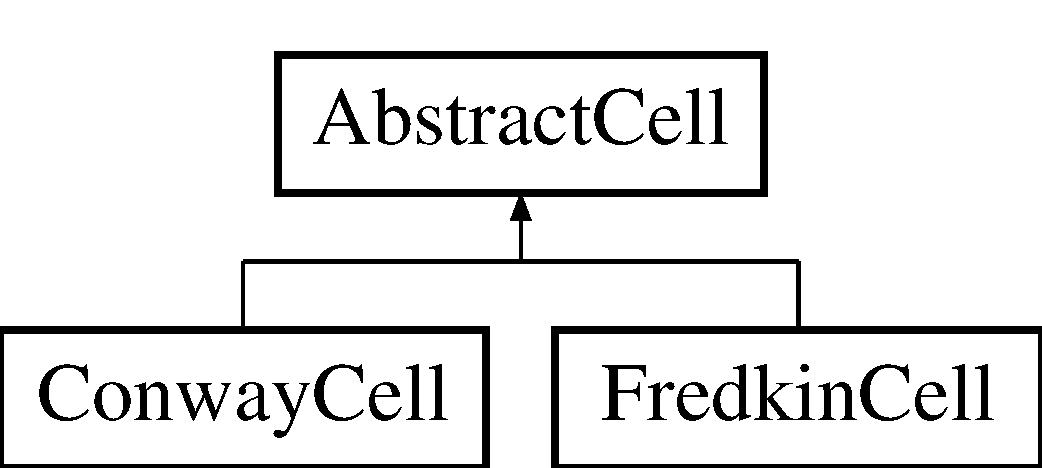
\includegraphics[height=2.000000cm]{classAbstractCell}
\end{center}
\end{figure}
\subsection*{Public Member Functions}
\begin{DoxyCompactItemize}
\item 
\hypertarget{classAbstractCell_ad799e7d9fed29d098293c76ac1dad5bb}{virtual bool {\bfseries is\-Alive} ()}\label{classAbstractCell_ad799e7d9fed29d098293c76ac1dad5bb}

\item 
\hypertarget{classAbstractCell_ae54b20831f27b0e867e68772f51b56c9}{virtual char {\bfseries is\-Status} ()}\label{classAbstractCell_ae54b20831f27b0e867e68772f51b56c9}

\item 
\hypertarget{classAbstractCell_a7f11cb2246a9360376a3c2b0bef3f97f}{virtual void {\bfseries cell\-\_\-\-Execute} (int neighs)}\label{classAbstractCell_a7f11cb2246a9360376a3c2b0bef3f97f}

\item 
\hypertarget{classAbstractCell_a6fd8f93b5a1547280fec2cb74241af38}{virtual \hyperlink{classAbstractCell}{Abstract\-Cell} $\ast$ {\bfseries clone} ()=0}\label{classAbstractCell_a6fd8f93b5a1547280fec2cb74241af38}

\end{DoxyCompactItemize}
\subsection*{Protected Member Functions}
\begin{DoxyCompactItemize}
\item 
\hypertarget{classAbstractCell_a9b400ff7731b2e3ede3a5a8a0c996a71}{{\bfseries F\-R\-I\-E\-N\-D\-\_\-\-T\-E\-S\-T} (Test\-Conway\-Contructor, conway1)}\label{classAbstractCell_a9b400ff7731b2e3ede3a5a8a0c996a71}

\item 
\hypertarget{classAbstractCell_a04c6d93c588a88ed67f8d7c94f375fe4}{{\bfseries F\-R\-I\-E\-N\-D\-\_\-\-T\-E\-S\-T} (Test\-Conway\-Contructor, conway2)}\label{classAbstractCell_a04c6d93c588a88ed67f8d7c94f375fe4}

\item 
\hypertarget{classAbstractCell_ae68e489f10b9223ced4f3bcad07ee4aa}{{\bfseries F\-R\-I\-E\-N\-D\-\_\-\-T\-E\-S\-T} (Test\-Fredkin\-Constructor, fred\-\_\-con1)}\label{classAbstractCell_ae68e489f10b9223ced4f3bcad07ee4aa}

\item 
\hypertarget{classAbstractCell_afd842743b9c9be674ff449acba1e1001}{{\bfseries F\-R\-I\-E\-N\-D\-\_\-\-T\-E\-S\-T} (Test\-Fredkin\-Constructor, fred\-\_\-con2)}\label{classAbstractCell_afd842743b9c9be674ff449acba1e1001}

\item 
\hypertarget{classAbstractCell_a8cda68b3384c84b181a1d575bfceb1df}{{\bfseries F\-R\-I\-E\-N\-D\-\_\-\-T\-E\-S\-T} (Test\-Fredkin\-Constructor, fred\-\_\-con3)}\label{classAbstractCell_a8cda68b3384c84b181a1d575bfceb1df}

\item 
\hypertarget{classAbstractCell_ae310a1a99ce0c001e73563d3615a73cf}{{\bfseries F\-R\-I\-E\-N\-D\-\_\-\-T\-E\-S\-T} (Test\-Conway\-Execute, c\-\_\-exe1)}\label{classAbstractCell_ae310a1a99ce0c001e73563d3615a73cf}

\item 
\hypertarget{classAbstractCell_abc78683e4bfbc60f28f8ac0b0d85de74}{{\bfseries F\-R\-I\-E\-N\-D\-\_\-\-T\-E\-S\-T} (Test\-Conway\-Execute, c\-\_\-exe2)}\label{classAbstractCell_abc78683e4bfbc60f28f8ac0b0d85de74}

\item 
\hypertarget{classAbstractCell_aa5c793e060395b153bcbcc0f7d496114}{{\bfseries F\-R\-I\-E\-N\-D\-\_\-\-T\-E\-S\-T} (Test\-Conway\-Execute, c\-\_\-exe3)}\label{classAbstractCell_aa5c793e060395b153bcbcc0f7d496114}

\item 
\hypertarget{classAbstractCell_a1b169f2f1ed4f3f9dcf811f6f0563547}{{\bfseries F\-R\-I\-E\-N\-D\-\_\-\-T\-E\-S\-T} (Test\-Fredkin\-Execute, f\-\_\-exe1)}\label{classAbstractCell_a1b169f2f1ed4f3f9dcf811f6f0563547}

\item 
\hypertarget{classAbstractCell_a4b37875c3a56d2c770ac8df9155ed513}{{\bfseries F\-R\-I\-E\-N\-D\-\_\-\-T\-E\-S\-T} (Test\-Fredkin\-Execute, f\-\_\-exe2)}\label{classAbstractCell_a4b37875c3a56d2c770ac8df9155ed513}

\item 
\hypertarget{classAbstractCell_a05687b0b9308abae21888164cec46d8b}{{\bfseries F\-R\-I\-E\-N\-D\-\_\-\-T\-E\-S\-T} (Test\-Fredkin\-Execute, f\-\_\-exe3)}\label{classAbstractCell_a05687b0b9308abae21888164cec46d8b}

\end{DoxyCompactItemize}
\subsection*{Protected Attributes}
\begin{DoxyCompactItemize}
\item 
\hypertarget{classAbstractCell_aa92e42d5bb67f3249d8e2dde2c3228e7}{bool {\bfseries alive}}\label{classAbstractCell_aa92e42d5bb67f3249d8e2dde2c3228e7}

\item 
\hypertarget{classAbstractCell_ad478280ffd92771aaa8e84bb48dd3d52}{char {\bfseries status}}\label{classAbstractCell_ad478280ffd92771aaa8e84bb48dd3d52}

\end{DoxyCompactItemize}


The documentation for this class was generated from the following files\-:\begin{DoxyCompactItemize}
\item 
Life.\-h\item 
Life.\-c++\end{DoxyCompactItemize}

\hypertarget{classCell}{\section{Cell Class Reference}
\label{classCell}\index{Cell@{Cell}}
}
\subsection*{Public Member Functions}
\begin{DoxyCompactItemize}
\item 
\hypertarget{classCell_af87eefd31ef08587611b6ad307a8a020}{{\bfseries Cell} (\hyperlink{classAbstractCell}{Abstract\-Cell} $\ast$ac)}\label{classCell_af87eefd31ef08587611b6ad307a8a020}

\item 
\hypertarget{classCell_a51f477d8039e209153054228a5792b0c}{{\bfseries Cell} (const \hyperlink{classCell}{Cell} \&c)}\label{classCell_a51f477d8039e209153054228a5792b0c}

\item 
\hypertarget{classCell_a0eb8254d3908d403f1475058178816f4}{{\bfseries Cell} (char b)}\label{classCell_a0eb8254d3908d403f1475058178816f4}

\item 
\hypertarget{classCell_a6c8a8a5b7fcc15c9ccea420e35374194}{bool {\bfseries is\-Alive} ()}\label{classCell_a6c8a8a5b7fcc15c9ccea420e35374194}

\item 
\hypertarget{classCell_a44a436396864079b7eddd1df256a93a6}{char {\bfseries is\-Status} ()}\label{classCell_a44a436396864079b7eddd1df256a93a6}

\item 
\hypertarget{classCell_a6aab96fba2b3c8659e8c6f7c4c17a9a6}{void {\bfseries cell\-\_\-\-Execute} (int n)}\label{classCell_a6aab96fba2b3c8659e8c6f7c4c17a9a6}

\item 
\hypertarget{classCell_ab0b7494a321cb288e900cab495b01daa}{\hyperlink{classCell}{Cell} \& {\bfseries operator=} (const \hyperlink{classCell}{Cell} \&c)}\label{classCell_ab0b7494a321cb288e900cab495b01daa}

\end{DoxyCompactItemize}
\subsection*{Friends}
\begin{DoxyCompactItemize}
\item 
\hypertarget{classCell_a89f0c180df69525f61cc2dfc08986171}{std\-::ostream \& {\bfseries operator$<$$<$} (std\-::ostream \&os, const \hyperlink{classCell}{Cell} \&sp)}\label{classCell_a89f0c180df69525f61cc2dfc08986171}

\end{DoxyCompactItemize}


The documentation for this class was generated from the following files\-:\begin{DoxyCompactItemize}
\item 
Life.\-h\item 
Life.\-c++\end{DoxyCompactItemize}

\hypertarget{classConwayCell}{\section{Conway\-Cell Class Reference}
\label{classConwayCell}\index{Conway\-Cell@{Conway\-Cell}}
}
Inheritance diagram for Conway\-Cell\-:\begin{figure}[H]
\begin{center}
\leavevmode
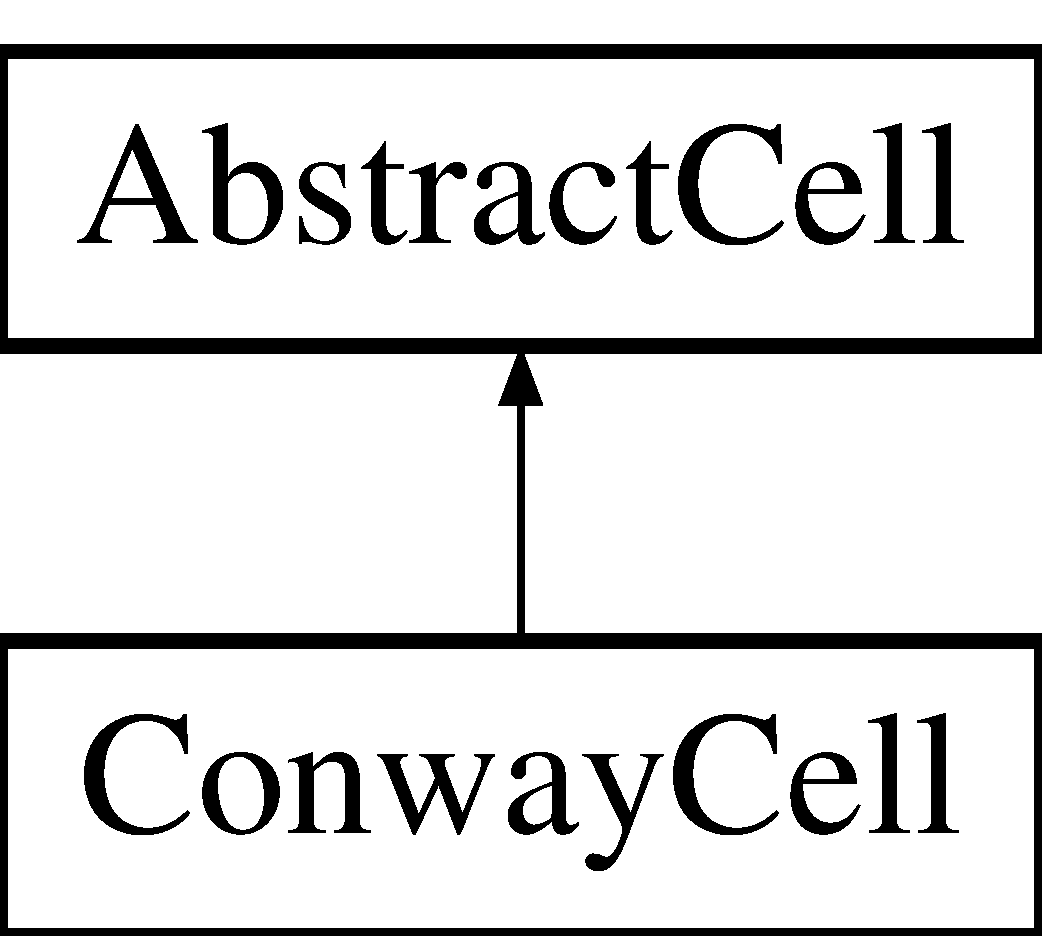
\includegraphics[height=2.000000cm]{classConwayCell}
\end{center}
\end{figure}
\subsection*{Public Member Functions}
\begin{DoxyCompactItemize}
\item 
\hypertarget{classConwayCell_a19d3407a2bf8febea7c97804d3f7e1c2}{{\bfseries Conway\-Cell} (char b)}\label{classConwayCell_a19d3407a2bf8febea7c97804d3f7e1c2}

\item 
\hypertarget{classConwayCell_a642f2c002fce9a1e39185f39cc5f65db}{\hyperlink{classAbstractCell}{Abstract\-Cell} $\ast$ {\bfseries clone} ()}\label{classConwayCell_a642f2c002fce9a1e39185f39cc5f65db}

\item 
\hypertarget{classConwayCell_a72890fcd4aec02ad47219914a510ecb3}{void {\bfseries cell\-\_\-\-Execute} (int n)}\label{classConwayCell_a72890fcd4aec02ad47219914a510ecb3}

\item 
\hypertarget{classConwayCell_a8431ae5417f7c05a8bf73b67c53d7140}{bool {\bfseries is\-Alive} ()}\label{classConwayCell_a8431ae5417f7c05a8bf73b67c53d7140}

\item 
\hypertarget{classConwayCell_aa6d025474d9c4b2cf8e57086989fed7e}{char {\bfseries is\-Status} ()}\label{classConwayCell_aa6d025474d9c4b2cf8e57086989fed7e}

\end{DoxyCompactItemize}
\subsection*{Friends}
\begin{DoxyCompactItemize}
\item 
\hypertarget{classConwayCell_a984780da7a7d6d3959f91581d28e340f}{std\-::ostream \& {\bfseries operator$<$$<$} (std\-::ostream \&os, const \hyperlink{classConwayCell}{Conway\-Cell} \&sp)}\label{classConwayCell_a984780da7a7d6d3959f91581d28e340f}

\end{DoxyCompactItemize}
\subsection*{Additional Inherited Members}


The documentation for this class was generated from the following files\-:\begin{DoxyCompactItemize}
\item 
Life.\-h\item 
Life.\-c++\end{DoxyCompactItemize}

\hypertarget{classFredkinCell}{\section{Fredkin\-Cell Class Reference}
\label{classFredkinCell}\index{Fredkin\-Cell@{Fredkin\-Cell}}
}
Inheritance diagram for Fredkin\-Cell\-:\begin{figure}[H]
\begin{center}
\leavevmode
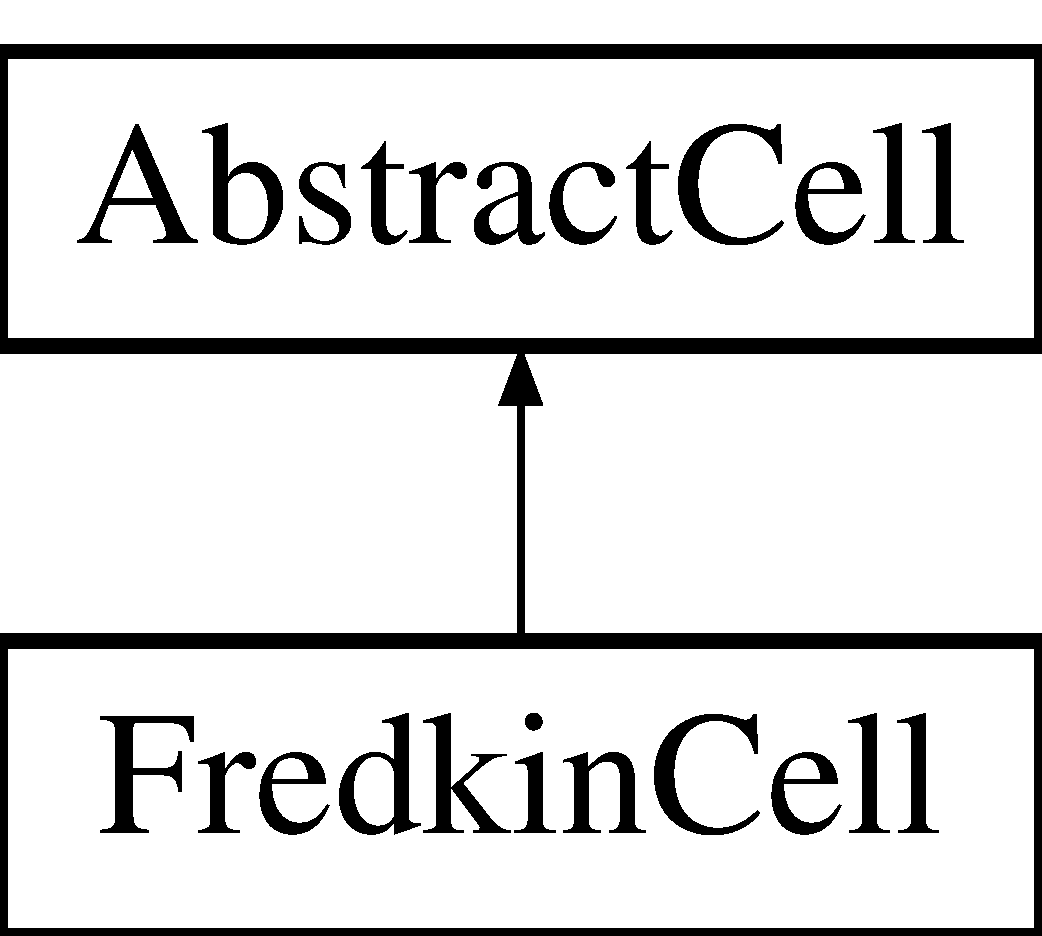
\includegraphics[height=2.000000cm]{classFredkinCell}
\end{center}
\end{figure}
\subsection*{Public Member Functions}
\begin{DoxyCompactItemize}
\item 
\hypertarget{classFredkinCell_a63acb9b6a4856b637b1475dd90958456}{{\bfseries Fredkin\-Cell} (char s)}\label{classFredkinCell_a63acb9b6a4856b637b1475dd90958456}

\item 
\hypertarget{classFredkinCell_a74d57ef05a09748127cb5b4a98c98192}{\hyperlink{classAbstractCell}{Abstract\-Cell} $\ast$ {\bfseries clone} ()}\label{classFredkinCell_a74d57ef05a09748127cb5b4a98c98192}

\item 
\hypertarget{classFredkinCell_a836097b769671606f7203961ddd8a52e}{bool {\bfseries is\-Alive} ()}\label{classFredkinCell_a836097b769671606f7203961ddd8a52e}

\item 
\hypertarget{classFredkinCell_a5e36ba49cec6b3570ebad41002cd43f6}{char {\bfseries is\-Status} ()}\label{classFredkinCell_a5e36ba49cec6b3570ebad41002cd43f6}

\item 
\hypertarget{classFredkinCell_a18ed9dbd44e9c89b38641dcfc20c147f}{void {\bfseries cell\-\_\-\-Execute} (int n)}\label{classFredkinCell_a18ed9dbd44e9c89b38641dcfc20c147f}

\end{DoxyCompactItemize}
\subsection*{Friends}
\begin{DoxyCompactItemize}
\item 
\hypertarget{classFredkinCell_a447820528b5f71838897a044f6e0c9b4}{std\-::ostream \& {\bfseries operator$<$$<$} (std\-::ostream \&os, const \hyperlink{classFredkinCell}{Fredkin\-Cell} \&sp)}\label{classFredkinCell_a447820528b5f71838897a044f6e0c9b4}

\end{DoxyCompactItemize}
\subsection*{Additional Inherited Members}


The documentation for this class was generated from the following files\-:\begin{DoxyCompactItemize}
\item 
Life.\-h\item 
Life.\-c++\end{DoxyCompactItemize}

\hypertarget{classLife}{\section{Life$<$ T $>$ Class Template Reference}
\label{classLife}\index{Life$<$ T $>$@{Life$<$ T $>$}}
}
\subsection*{Public Member Functions}
\begin{DoxyCompactItemize}
\item 
\hypertarget{classLife_a54b6624b13387f6e38df5ecd9f766d16}{void {\bfseries parse\-File} (istream \&r)}\label{classLife_a54b6624b13387f6e38df5ecd9f766d16}

\item 
\hypertarget{classLife_ade3bb83f54dbe14cba1b39e72a0b868f}{int {\bfseries alive\-\_\-neighs} (int x, int y)}\label{classLife_ade3bb83f54dbe14cba1b39e72a0b868f}

\item 
\hypertarget{classLife_a1999b45983564672f38003a484e4958b}{void {\bfseries print\-Grid} ()}\label{classLife_a1999b45983564672f38003a484e4958b}

\item 
\hypertarget{classLife_a82a483ffd963a337bfa8047743dca111}{void {\bfseries execute} ()}\label{classLife_a82a483ffd963a337bfa8047743dca111}

\item 
\hypertarget{classLife_a066f96b1d5434e573a35cf6505c33685}{void {\bfseries run} (int iter, int nums)}\label{classLife_a066f96b1d5434e573a35cf6505c33685}

\item 
\hypertarget{classLife_a5a8da0f57542daabc1712a826c13b051}{int {\bfseries get\-Population} ()}\label{classLife_a5a8da0f57542daabc1712a826c13b051}

\item 
\hypertarget{classLife_a0671eb7c9ecfb698ce14bb48f710e7e6}{{\bfseries Life} (int x, int y)}\label{classLife_a0671eb7c9ecfb698ce14bb48f710e7e6}

\end{DoxyCompactItemize}


The documentation for this class was generated from the following file\-:\begin{DoxyCompactItemize}
\item 
Life.\-h\end{DoxyCompactItemize}

%--- End generated contents ---

% Index
\newpage
\phantomsection
\addcontentsline{toc}{chapter}{Index}
\printindex

\end{document}
